
%% bare_jrnl.tex
%% V1.4a
%% 2014/09/17
%% by Michael Shell
%% see http://www.michaelshell.org/
%% for current contact information.
%%
%% This is a skeleton file demonstrating the use of IEEEtran.cls
%% (requires IEEEtran.cls version 1.8a or later) with an IEEE
%% journal paper.
%%
%% Support sites:
%% http://www.michaelshell.org/tex/ieeetran/
%% http://www.ctan.org/tex-archive/macros/latex/contrib/IEEEtran/
%% and
%% http://www.ieee.org/

%%*************************************************************************
%% Legal Notice:
%% This code is offered as-is without any warranty either expressed or
%% implied; without even the implied warranty of MERCHANTABILITY or
%% FITNESS FOR A PARTICULAR PURPOSE! 
%% User assumes all risk.
%% In no event shall IEEE or any contributor to this code be liable for
%% any damages or losses, including, but not limited to, incidental,
%% consequential, or any other damages, resulting from the use or misuse
%% of any information contained here.
%%
%% All comments are the opinions of their respective authors and are not
%% necessarily endorsed by the IEEE.
%%
%% This work is distributed under the LaTeX Project Public License (LPPL)
%% ( http://www.latex-project.org/ ) version 1.3, and may be freely used,
%% distributed and modified. A copy of the LPPL, version 1.3, is included
%% in the base LaTeX documentation of all distributions of LaTeX released
%% 2003/12/01 or later.
%% Retain all contribution notices and credits.
%% ** Modified files should be clearly indicated as such, including  **
%% ** renaming them and changing author support contact information. **
%%
%% File list of work: IEEEtran.cls, IEEEtran_HOWTO.pdf, bare_adv.tex,
%%                    bare_conf.tex, bare_jrnl.tex, bare_conf_compsoc.tex,
%%                    bare_jrnl_compsoc.tex, bare_jrnl_transmag.tex
%%*************************************************************************


% *** Authors should verify (and, if needed, correct) their LaTeX system  ***
% *** with the testflow diagnostic prior to trusting their LaTeX platform ***
% *** with production work. IEEE's font choices and paper sizes can       ***
% *** trigger bugs that do not appear when using other class files.       ***                          ***
% The testflow support page is at:
% http://www.michaelshell.org/tex/testflow/



\documentclass[journal]{IEEEtran}
%
% If IEEEtran.cls has not been installed into the LaTeX system files,
% manually specify the path to it like:
% \documentclass[journal]{../sty/IEEEtran}





% Some very useful LaTeX packages include:
% (uncomment the ones you want to load)


% *** MISC UTILITY PACKAGES ***
%
%\usepackage{ifpdf}
% Heiko Oberdiek's ifpdf.sty is very useful if you need conditional
% compilation based on whether the output is pdf or dvi.
% usage:
% \ifpdf
%   % pdf code
% \else
%   % dvi code
% \fi
% The latest version of ifpdf.sty can be obtained from:
% http://www.ctan.org/tex-archive/macros/latex/contrib/oberdiek/
% Also, note that IEEEtran.cls V1.7 and later provides a builtin
% \ifCLASSINFOpdf conditional that works the same way.
% When switching from latex to pdflatex and vice-versa, the compiler may
% have to be run twice to clear warning/error messages.






% *** CITATION PACKAGES ***
%
%\usepackage{cite}
% cite.sty was written by Donald Arseneau
% V1.6 and later of IEEEtran pre-defines the format of the cite.sty package
% \cite{} output to follow that of IEEE. Loading the cite package will
% result in citation numbers being automatically sorted and properly
% "compressed/ranged". e.g., [1], [9], [2], [7], [5], [6] without using
% cite.sty will become [1], [2], [5]--[7], [9] using cite.sty. cite.sty's
% \cite will automatically add leading space, if needed. Use cite.sty's
% noadjust option (cite.sty V3.8 and later) if you want to turn this off
% such as if a citation ever needs to be enclosed in parenthesis.
% cite.sty is already installed on most LaTeX systems. Be sure and use
% version 5.0 (2009-03-20) and later if using hyperref.sty.
% The latest version can be obtained at:
% http://www.ctan.org/tex-archive/macros/latex/contrib/cite/
% The documentation is contained in the cite.sty file itself.






% *** GRAPHICS RELATED PACKAGES ***
%
\ifCLASSINFOpdf
   \usepackage[pdftex]{graphicx}
  % declare the path(s) where your graphic files are
  % \graphicspath{{../pdf/}{../jpeg/}}
  % and their extensions so you won't have to specify these with
  % every instance of \includegraphics
  % \DeclareGraphicsExtensions{.pdf,.jpeg,.png}
\else
  % or other class option (dvipsone, dvipdf, if not using dvips). graphicx
  % will default to the driver specified in the system graphics.cfg if no
  % driver is specified.
  % \usepackage[dvips]{graphicx}
  % declare the path(s) where your graphic files are
  % \graphicspath{{../eps/}}
  % and their extensions so you won't have to specify these with
  % every instance of \includegraphics
  % \DeclareGraphicsExtensions{.eps}
\fi
% graphicx was written by David Carlisle and Sebastian Rahtz. It is
% required if you want graphics, photos, etc. graphicx.sty is already
% installed on most LaTeX systems. The latest version and documentation
% can be obtained at: 
% http://www.ctan.org/tex-archive/macros/latex/required/graphics/
% Another good source of documentation is "Using Imported Graphics in
% LaTeX2e" by Keith Reckdahl which can be found at:
% http://www.ctan.org/tex-archive/info/epslatex/
%
% latex, and pdflatex in dvi mode, support graphics in encapsulated
% postscript (.eps) format. pdflatex in pdf mode supports graphics
% in .pdf, .jpeg, .png and .mps (metapost) formats. Users should ensure
% that all non-photo figures use a vector format (.eps, .pdf, .mps) and
% not a bitmapped formats (.jpeg, .png). IEEE frowns on bitmapped formats
% which can result in "jaggedy"/blurry rendering of lines and letters as
% well as large increases in file sizes.
%
% You can find documentation about the pdfTeX application at:
% http://www.tug.org/applications/pdftex





% *** MATH PACKAGES ***
%
\usepackage[cmex10]{amsmath}
% A popular package from the American Mathematical Society that provides
% many useful and powerful commands for dealing with mathematics. If using
% it, be sure to load this package with the cmex10 option to ensure that
% only type 1 fonts will utilized at all point sizes. Without this option,
% it is possible that some math symbols, particularly those within
% footnotes, will be rendered in bitmap form which will result in a
% document that can not be IEEE Xplore compliant!
%
% Also, note that the amsmath package sets \interdisplaylinepenalty to 10000
% thus preventing page breaks from occurring within multiline equations. Use:
%\interdisplaylinepenalty=2500
% after loading amsmath to restore such page breaks as IEEEtran.cls normally
% does. amsmath.sty is already installed on most LaTeX systems. The latest
% version and documentation can be obtained at:
% http://www.ctan.org/tex-archive/macros/latex/required/amslatex/math/





% *** SPECIALIZED LIST PACKAGES ***
%
%\usepackage{algorithmic}
% algorithmic.sty was written by Peter Williams and Rogerio Brito.
% This package provides an algorithmic environment fo describing algorithms.
% You can use the algorithmic environment in-text or within a figure
% environment to provide for a floating algorithm. Do NOT use the algorithm
% floating environment provided by algorithm.sty (by the same authors) or
% algorithm2e.sty (by Christophe Fiorio) as IEEE does not use dedicated
% algorithm float types and packages that provide these will not provide
% correct IEEE style captions. The latest version and documentation of
% algorithmic.sty can be obtained at:
% http://www.ctan.org/tex-archive/macros/latex/contrib/algorithms/
% There is also a support site at:
% http://algorithms.berlios.de/index.html
% Also of interest may be the (relatively newer and more customizable)
% algorithmicx.sty package by Szasz Janos:
% http://www.ctan.org/tex-archive/macros/latex/contrib/algorithmicx/




% *** ALIGNMENT PACKAGES ***
%
%\usepackage{array}
% Frank Mittelbach's and David Carlisle's array.sty patches and improves
% the standard LaTeX2e array and tabular environments to provide better
% appearance and additional user controls. As the default LaTeX2e table
% generation code is lacking to the point of almost being broken with
% respect to the quality of the end results, all users are strongly
% advised to use an enhanced (at the very least that provided by array.sty)
% set of table tools. array.sty is already installed on most systems. The
% latest version and documentation can be obtained at:
% http://www.ctan.org/tex-archive/macros/latex/required/tools/


% IEEEtran contains the IEEEeqnarray family of commands that can be used to
% generate multiline equations as well as matrices, tables, etc., of high
% quality.




% *** SUBFIGURE PACKAGES ***
%\ifCLASSOPTIONcompsoc
%  \usepackage[caption=false,font=normalsize,labelfont=sf,textfont=sf]{subfig}
%\else
%  \usepackage[caption=false,font=footnotesize]{subfig}
%\fi
% subfig.sty, written by Steven Douglas Cochran, is the modern replacement
% for subfigure.sty, the latter of which is no longer maintained and is
% incompatible with some LaTeX packages including fixltx2e. However,
% subfig.sty requires and automatically loads Axel Sommerfeldt's caption.sty
% which will override IEEEtran.cls' handling of captions and this will result
% in non-IEEE style figure/table captions. To prevent this problem, be sure
% and invoke subfig.sty's "caption=false" package option (available since
% subfig.sty version 1.3, 2005/06/28) as this is will preserve IEEEtran.cls
% handling of captions.
% Note that the Computer Society format requires a larger sans serif font
% than the serif footnote size font used in traditional IEEE formatting
% and thus the need to invoke different subfig.sty package options depending
% on whether compsoc mode has been enabled.
%
% The latest version and documentation of subfig.sty can be obtained at:
% http://www.ctan.org/tex-archive/macros/latex/contrib/subfig/




% *** FLOAT PACKAGES ***
%
%\usepackage{fixltx2e}
% fixltx2e, the successor to the earlier fix2col.sty, was written by
% Frank Mittelbach and David Carlisle. This package corrects a few problems
% in the LaTeX2e kernel, the most notable of which is that in current
% LaTeX2e releases, the ordering of single and double column floats is not
% guaranteed to be preserved. Thus, an unpatched LaTeX2e can allow a
% single column figure to be placed prior to an earlier double column
% figure. The latest version and documentation can be found at:
% http://www.ctan.org/tex-archive/macros/latex/base/


%\usepackage{stfloats}
% stfloats.sty was written by Sigitas Tolusis. This package gives LaTeX2e
% the ability to do double column floats at the bottom of the page as well
% as the top. (e.g., "\begin{figure*}[!b]" is not normally possible in
% LaTeX2e). It also provides a command:
%\fnbelowfloat
% to enable the placement of footnotes below bottom floats (the standard
% LaTeX2e kernel puts them above bottom floats). This is an invasive package
% which rewrites many portions of the LaTeX2e float routines. It may not work
% with other packages that modify the LaTeX2e float routines. The latest
% version and documentation can be obtained at:
% http://www.ctan.org/tex-archive/macros/latex/contrib/sttools/
% Do not use the stfloats baselinefloat ability as IEEE does not allow
% \baselineskip to stretch. Authors submitting work to the IEEE should note
% that IEEE rarely uses double column equations and that authors should try
% to avoid such use. Do not be tempted to use the cuted.sty or midfloat.sty
% packages (also by Sigitas Tolusis) as IEEE does not format its papers in
% such ways.
% Do not attempt to use stfloats with fixltx2e as they are incompatible.
% Instead, use Morten Hogholm'a dblfloatfix which combines the features
% of both fixltx2e and stfloats:
%
% \usepackage{dblfloatfix}
% The latest version can be found at:
% http://www.ctan.org/tex-archive/macros/latex/contrib/dblfloatfix/




%\ifCLASSOPTIONcaptionsoff
%  \usepackage[nomarkers]{endfloat}
% \let\MYoriglatexcaption\caption
% \renewcommand{\caption}[2][\relax]{\MYoriglatexcaption[#2]{#2}}
%\fi
% endfloat.sty was written by James Darrell McCauley, Jeff Goldberg and 
% Axel Sommerfeldt. This package may be useful when used in conjunction with 
% IEEEtran.cls'  captionsoff option. Some IEEE journals/societies require that
% submissions have lists of figures/tables at the end of the paper and that
% figures/tables without any captions are placed on a page by themselves at
% the end of the document. If needed, the draftcls IEEEtran class option or
% \CLASSINPUTbaselinestretch interface can be used to increase the line
% spacing as well. Be sure and use the nomarkers option of endfloat to
% prevent endfloat from "marking" where the figures would have been placed
% in the text. The two hack lines of code above are a slight modification of
% that suggested by in the endfloat docs (section 8.4.1) to ensure that
% the full captions always appear in the list of figures/tables - even if
% the user used the short optional argument of \caption[]{}.
% IEEE papers do not typically make use of \caption[]'s optional argument,
% so this should not be an issue. A similar trick can be used to disable
% captions of packages such as subfig.sty that lack options to turn off
% the subcaptions:
% For subfig.sty:
% \let\MYorigsubfloat\subfloat
% \renewcommand{\subfloat}[2][\relax]{\MYorigsubfloat[]{#2}}
% However, the above trick will not work if both optional arguments of
% the \subfloat command are used. Furthermore, there needs to be a
% description of each subfigure *somewhere* and endfloat does not add
% subfigure captions to its list of figures. Thus, the best approach is to
% avoid the use of subfigure captions (many IEEE journals avoid them anyway)
% and instead reference/explain all the subfigures within the main caption.
% The latest version of endfloat.sty and its documentation can obtained at:
% http://www.ctan.org/tex-archive/macros/latex/contrib/endfloat/
%
% The IEEEtran \ifCLASSOPTIONcaptionsoff conditional can also be used
% later in the document, say, to conditionally put the References on a 
% page by themselves.




% *** PDF, URL AND HYPERLINK PACKAGES ***
%
%\usepackage{url}
% url.sty was written by Donald Arseneau. It provides better support for
% handling and breaking URLs. url.sty is already installed on most LaTeX
% systems. The latest version and documentation can be obtained at:
% http://www.ctan.org/tex-archive/macros/latex/contrib/url/
% Basically, \url{my_url_here}.




% *** Do not adjust lengths that control margins, column widths, etc. ***
% *** Do not use packages that alter fonts (such as pslatex).         ***
% There should be no need to do such things with IEEEtran.cls V1.6 and later.
% (Unless specifically asked to do so by the journal or conference you plan
% to submit to, of course. )


% correct bad hyphenation here
\hyphenation{op-tical net-works semi-conduc-tor}


\begin{document}
%
% paper title
% Titles are generally capitalized except for words such as a, an, and, as,
% at, but, by, for, in, nor, of, on, or, the, to and up, which are usually
% not capitalized unless they are the first or last word of the title.
% Linebreaks \\ can be used within to get better formatting as desired.
% Do not put math or special symbols in the title.
\title{Bare Demo of IEEEtran.cls for Journals}
%
%
% author names and IEEE memberships
% note positions of commas and nonbreaking spaces ( ~ ) LaTeX will not break
% a structure at a ~ so this keeps an author's name from being broken across
% two lines.
% use \thanks{} to gain access to the first footnote area
% a separate \thanks must be used for each paragraph as LaTeX2e's \thanks
% was not built to handle multiple paragraphs
%

\author{Michael~Shell,~\IEEEmembership{Member,~IEEE,}
        John~Doe,~\IEEEmembership{Fellow,~OSA,}
        and~Jane~Doe,~\IEEEmembership{Life~Fellow,~IEEE}% <-this % stops a space
\thanks{M. Shell is with the Department
of Electrical and Computer Engineering, Georgia Institute of Technology, Atlanta,
GA, 30332 USA e-mail: (see http://www.michaelshell.org/contact.html).}% <-this % stops a space
\thanks{J. Doe and J. Doe are with Anonymous University.}% <-this % stops a space
\thanks{Manuscript received April 19, 2005; revised September 17, 2014.}}

% note the % following the last \IEEEmembership and also \thanks - 
% these prevent an unwanted space from occurring between the last author name
% and the end of the author line. i.e., if you had this:
% 
% \author{....lastname \thanks{...} \thanks{...} }
%                     ^------------^------------^----Do not want these spaces!
%
% a space would be appended to the last name and could cause every name on that
% line to be shifted left slightly. This is one of those "LaTeX things". For
% instance, "\textbf{A} \textbf{B}" will typeset as "A B" not "AB". To get
% "AB" then you have to do: "\textbf{A}\textbf{B}"
% \thanks is no different in this regard, so shield the last } of each \thanks
% that ends a line with a % and do not let a space in before the next \thanks.
% Spaces after \IEEEmembership other than the last one are OK (and needed) as
% you are supposed to have spaces between the names. For what it is worth,
% this is a minor point as most people would not even notice if the said evil
% space somehow managed to creep in.



% The paper headers
\markboth{Journal of \LaTeX\ Class Files,~Vol.~13, No.~9, September~2014}%
{Shell \MakeLowercase{\textit{et al.}}: Bare Demo of IEEEtran.cls for Journals}
% The only time the second header will appear is for the odd numbered pages
% after the title page when using the twoside option.
% 
% *** Note that you probably will NOT want to include the author's ***
% *** name in the headers of peer review papers.                   ***
% You can use \ifCLASSOPTIONpeerreview for conditional compilation here if
% you desire.




% If you want to put a publisher's ID mark on the page you can do it like
% this:
%\IEEEpubid{0000--0000/00\$00.00~\copyright~2014 IEEE}
% Remember, if you use this you must call \IEEEpubidadjcol in the second
% column for its text to clear the IEEEpubid mark.



% use for special paper notices
%\IEEEspecialpapernotice{(Invited Paper)}




% make the title area
\maketitle

% As a general rule, do not put math, special symbols or citations
% in the abstract or keywords.
\begin{abstract}
Genetically identical cells express their genes at different labels and respond differently to changes in their environment.  Large-scale microscopy-based experiments are needed to characterize the dynamics of such cell-to-cell variability as well as the phenotypic diversity in response to perturbations in growth conditions. The rich data from image-based experiments requires robust and efficient analysis. In this work, we analyze bacterial cells growing in monolayers in a microfluidic device. Individual cells are identified using a novel curvature based approach and tracked over time for several generations. The resulting tracks are thereafter assessed and sorted based on track quality to reduce errors in subsequent analysis of bacterial growth rates. The proposed method performs better than the state-of-the-art methods for segmenting phase contrast and fluorescent images, and we show a 10-fold increase in analysis speed.
\end{abstract}

% Note that keywords are not normally used for peerreview papers.
\begin{IEEEkeywords}
IEEEtran, journal, \LaTeX, paper, template.
\end{IEEEkeywords}






% For peer review papers, you can put extra information on the cover
% page as needed:
% \ifCLASSOPTIONpeerreview
% \begin{center} \bfseries EDICS Category: 3-BBND \end{center}
% \fi
%
% For peerreview papers, this IEEEtran command inserts a page break and
% creates the second title. It will be ignored for other modes.
\IEEEpeerreviewmaketitle



\section{Introduction}
% The very first letter is a 2 line initial drop letter followed
% by the rest of the first word in caps.
% 
% form to use if the first word consists of a single letter:
% \IEEEPARstart{A}{demo} file is ....
% 
% form to use if you need the single drop letter followed by
% normal text (unknown if ever used by IEEE):
% \IEEEPARstart{A}{}demo file is ....
% 
% Some journals put the first two words in caps:
% \IEEEPARstart{T}{his demo} file is ....
% 
% Here we have the typical use of a "T" for an initial drop letter
% and "HIS" in caps to complete the first word.
\IEEEPARstart{L}{ive} cell experiments pave the way to understand the complex biological functions of living organisms. Many live cell experiments require monitoring of cells under different conditions over several generations. Isogenic cells display cell-to-cell variability even when grown under similar conditions \cite{elowitzstochastic2002}. To study the origin and consequences of such variation it is necessary to monitor many individual cells for extended periods of time to reach statistically verifiable conclusions \cite{yuichiquantify2010}. Time-lapse experiments usually generate large quantities of data, which become extremely difficult for human observers to evaluate in an unbiased way \cite{qiangmicroscope2008}. Thus, automated systems are necessary to analyze such datasets in order to to reach robust and reproducible results. 

Time-lapse imaging of growing bacterial cells are important both to answer fundamental biological questions related to the bacterial cell cycle as well as to study response to changes in growth condition due to changes in nutrients or antibiotics. Based on the growth conditions and imaging modalities, various automated image segmentation and tracking packages have been created. MicrobeTracker \cite {sliusarenkohigh2011} was designed to segment phase contrast images and detect fluorescent spots in a parallel fluorescent channel. Schnitzcells was specifically designed to analyze fluorescent time-lapse images of E. coli grown on agarose \cite  {youngmeasuring2012}, and MAMLE \cite {chowdhurycell2013} was also designed to analyze E. coli from phase contrast and fluorescent images.

Most image segmentation methods rely on raw pixel intensities to get an initial segmentation result, and further refined segmentation depends on this initial segmentation. MicrobeTracker \cite {sliusarenkohigh2011} finds an initial segmentation using Otsu’s thresholding method \cite {otsuthreshold1979} followed by edge detection and watershed segmentation. In the final step, active contours are applied to refine object boundaries. MicrobeTracker needs manual correction of the first frame to get satisfactory segmentation results for time-lapse images. It is difficult to analyze large image sequences in MicrobeTracker due to its inherent memory problems, and it is often necessary to modify the code for practical applications. MAMLE \cite {chowdhurycell2013} uses range filtering to find an initial segmentation result, followed by multi-scale edge detection and a maximum likelihood classification to correct over- and under- segmentation. In Schnitzcells \cite {youngmeasuring2012}, initial segmentation is achieved by edge detection followed by post processing to correct segmentation errors. 

Phase contrast images of E. coli exhibit high-intensity regions inside cellular regions comparable to, or even brighter than, regions between cells. Relying on raw intensity therefore leads to over- and under-segmentation at the same time. The problem becomes amplified when trying to track cells over time. Even a 1\% error in detection of cells in every frame renders the cell lineage useless for further analysis if many cells are tracked over a long time.

Previously published cell tracking algorithms rely on model evolution, where a model of the cell is evolved over time using techniques such as active contour models \cite {zimmersegmentation2002} or level sets \cite {dzyubachykadvanced2010}, and tracking by detection \cite {bisereliable2011}. Tracking by detection involves two stages; segmentation and tracking. Sometimes both these steps are combined together to get final tracking result \cite {jugoptimal2014}. 

In this work, we use tracking by detection, i.e., separate the segmentation and tracking problems and solve them separately, followed by a quality control and refinement step where some of the segmentation and tracking errors are corrected. Cell segmentation is done using our novel Curvature Based Approach, hereafter called as CBA, and tracking is done using a state-of-the-art tracking algorithm \cite {magnussonglobal2014}. In the following sections we present our segmentation methodology and compare it with that of MicrobeTracker and MAMLE on phase contrast as well as fluorescence images, from our own and previously published experiments. After segmentation, we track the cells through the time-lapse sequence and then perform post tracking segmentation correction to get a final segmentation result. Finally, we show how the combined segmentation and tracking approach can be applied to quantify differences in cell growth rate under different experimental conditions.

\section{Methodology}
\subsection{Image Acquisition}
The bacterial cell colonies in our own experiments were grown on a specially designed microfluidic device in Polydimethylsiloxane(PDMS)\cite {ullmanhigh2012} with a growth chamber, a “trap”, of size 40 x 40 x 0.9 μm, which is open to growth media exchange at two ends.  The cells grow in a single layer and as the size of the microcolony gets larger than the trap, excess cells leave the trap through the outlet, thus maintaining the colony size of approximately 200 cells nearly constant throughout the experiment. Images were captured using an inverted microscope fitted with separate cameras for phase contrast and fluorescent channels. The microscope is equipped with a TIR based hardware autofocus that keeps the cells in focus over days. 51 traps can be monitored in parallel and growth conditions can be changed in 2s \cite{hammarlac2012} using computer controlled pumps. Phase contrast images were acquired every 30 or 60 seconds at 125 ms exposure time using CFW-1312M (Scion Corporation) and fluorescent images were acquired every 60 seconds using an EMCCD camera (Andor Technologies) and DPSS laser excitation at 514 nm (Coherent). The MG1655 bacteria are grown in M9 media supplemented with glucose or glycerol for growth rate comparison and amino acids. The fluorescent cells express turboRFP constitutively from a chromosomally integrated promoter. Bacterial cell colonies from the MicrobeTracker and Schnitzcells datasets were grown as described in \cite {sliusarenkohigh2011} and \cite {youngmeasuring2012}.

% needed in second column of first page if using \IEEEpubid
%\IEEEpubidadjcol
\subsection{Image Preprocessing }
The input images are of size 1360x1024 pixels and contain the cell colony as well as some regions of the microfluidic device. We aligned the image sequences based on image cross correlation to account for the stage repositioning inaccuracy that occurred when cycling though different traps during the image acquisition process. The aligned images were manually cropped to the cellular region. Since the stack was aligned, manual selection on the first frame was enough to crop the entire image stack.

\subsection{Curvature Based Contrast Enhancement }
In the input phase contrast images, the E. coli cells appear as dark rod-shaped objects on a brighter background \ref {figure 2a}. The E. coli colony is tightly packed so that the intensity values between the cells are often similar to those inside the cells, and it is common to see high intensity regions inside cells, meaning that any purely intensity based approach for segmentation will result in erroneous output. However, we have observed that there is a general intensity variation that is occurring between the cells. To detect these regions of intensity variation, we used the separation of principal curvature of the intensity surface \cite {willmoreintroduction1959}. The regions were thereafter separated based on the minimal curvature as described below. 

The curvature was found using techniques from differential geometry \cite  {willmoreintroduction1959}. Consider a 1D case, where \textbf{r} is a curve as shown in ref Figure 1 and p and q are two points on the curve. We know that the gradient of the curve with respect to the arc length gives the tangent, t, at that point, i.e., t = r’. The rate of change of tangent direction as we move along the curve is the curvature of the curve, i.e., t’ = kn, where n is the unit normal vector to the curve that is perpendicular to the tangent and k is the curvature. So we have r” = kn. This shows that the curvature at a point is the second derivative of the curve at that point.  The sign of the curvature is determined by whether the slope is increasing or decreasing. Here we can see that it is negative in the maximum point and positive in the minimum point as shown by kp and kq (arrow pointing upward as positive and arrow pointing downward as negative).
\begin{figure}[t ]
	\begin{center}
		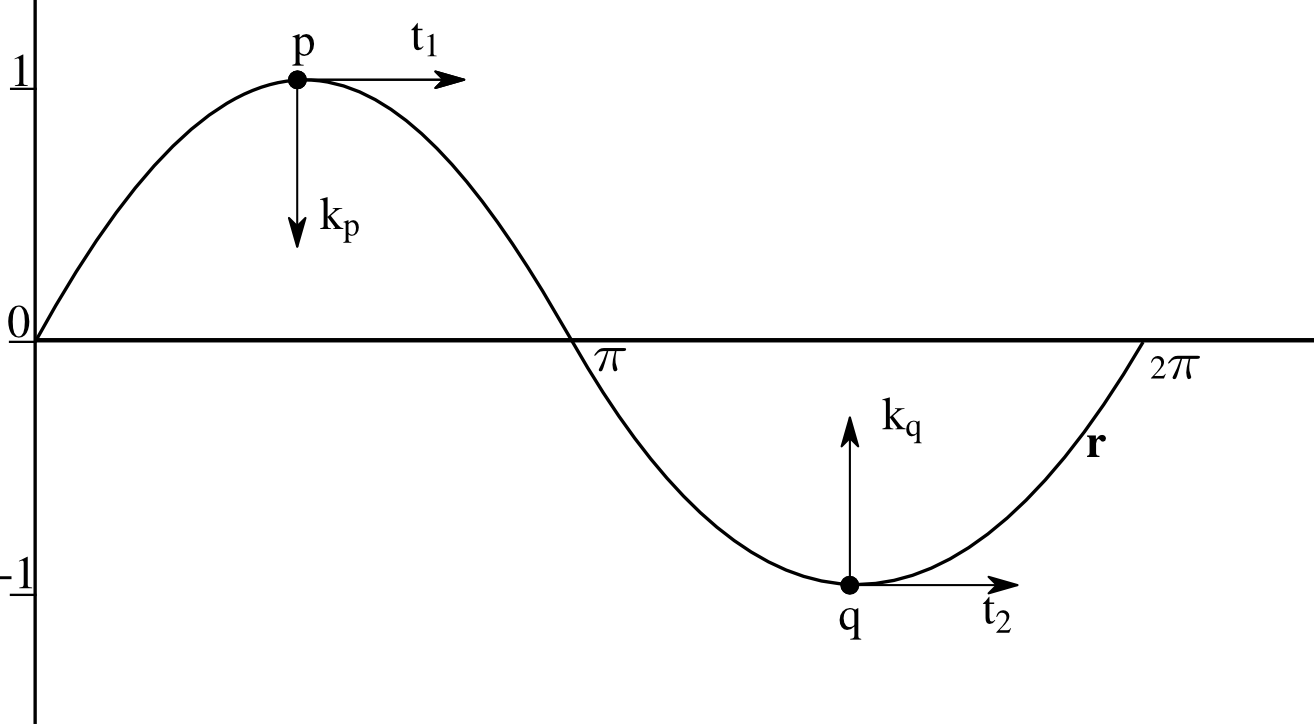
\includegraphics[width=45mm]{fig1cuve.png}
		\caption{$k_p$ is the curvature at point \textit{p} with negative value and $k_q$ is the curvature at point \textit{q} with positive value for the curve \textbf{r}}
		\label{fig:curve}
	\end{center}    
\end{figure}
We extended the same idea to the 2D case. Consider a gray scale image as a surface in 3D with (x,y) being the spatial coordinates and I(x,y) being the gray level intensity at that particular spatial location. Following a similar convention as for the 1D case, the image surface is assumed to be continuous with partial derivatives existing at least to order 2 \cite {willmoreintroduction1959}. Here, we first made the image smooth by convolving it with a Gaussian kernel. We set the standard deviation of the Gaussian to 1.4 pixels, which is approximately 1/10th the width of the E. coli cells, found experimentally.


A particular point on the image surface has an infinite number of curves passing through it. Out of all these curves there are two curves that are particularly interesting. They are the curve with maximum curvature and the curve with minimum curvature. These curves are orthogonal to each other. These curvatures are equal to the eigenvalues of the Hessian matrix \cite {thorpeelementary1979}. The Hessian is the second derivative matrix of the image, calculated for every pixels, which is created as H = [[Ixx, Ixy][Ixy Iyy]], where Ixx and Iyy are the 2nd derivatives of the image taken in the x- and y-directions, and Ixy is the derivative of the image taken first in the x-direction and then in the y-direction, using discrete approximations \cite{woodfordnumerical2012}. The eigenvalues can be calculated as follows 


\begin{equation}
k_{1,2} = \frac{trace(H)\pm \sqrt{trace(H)^2 -4\times det(H)} }{2}
\end{equation}
Here, k1 and k2 are the principal curvatures with k1<k2.  In phase contrast images of E. coli, consider two rod shaped cells lying parallel to each other, the cells are dark and the region between the cells is bright. When we calculate principal curvatures in region between the cells, one is perpendicular to the major axis of the cell and its curvature is negative and the other one parallel to the major axis of the cell is zero or small value near zero (positive or negative depending on local intensity values). Taking the lowest value of the two gives the curve with the greatest curvature magnitude in the negative direction at that point. In this way we can enhance the contrast of the image in bright background regions between cells while avoiding enhancing variations inside the darker cell regions, as shown in Figure \ref{fig:contrastenhance}. 

\begin{figure}[h]
	\begin{center}
		\begin{tabular}{ccc}
			%\hline
			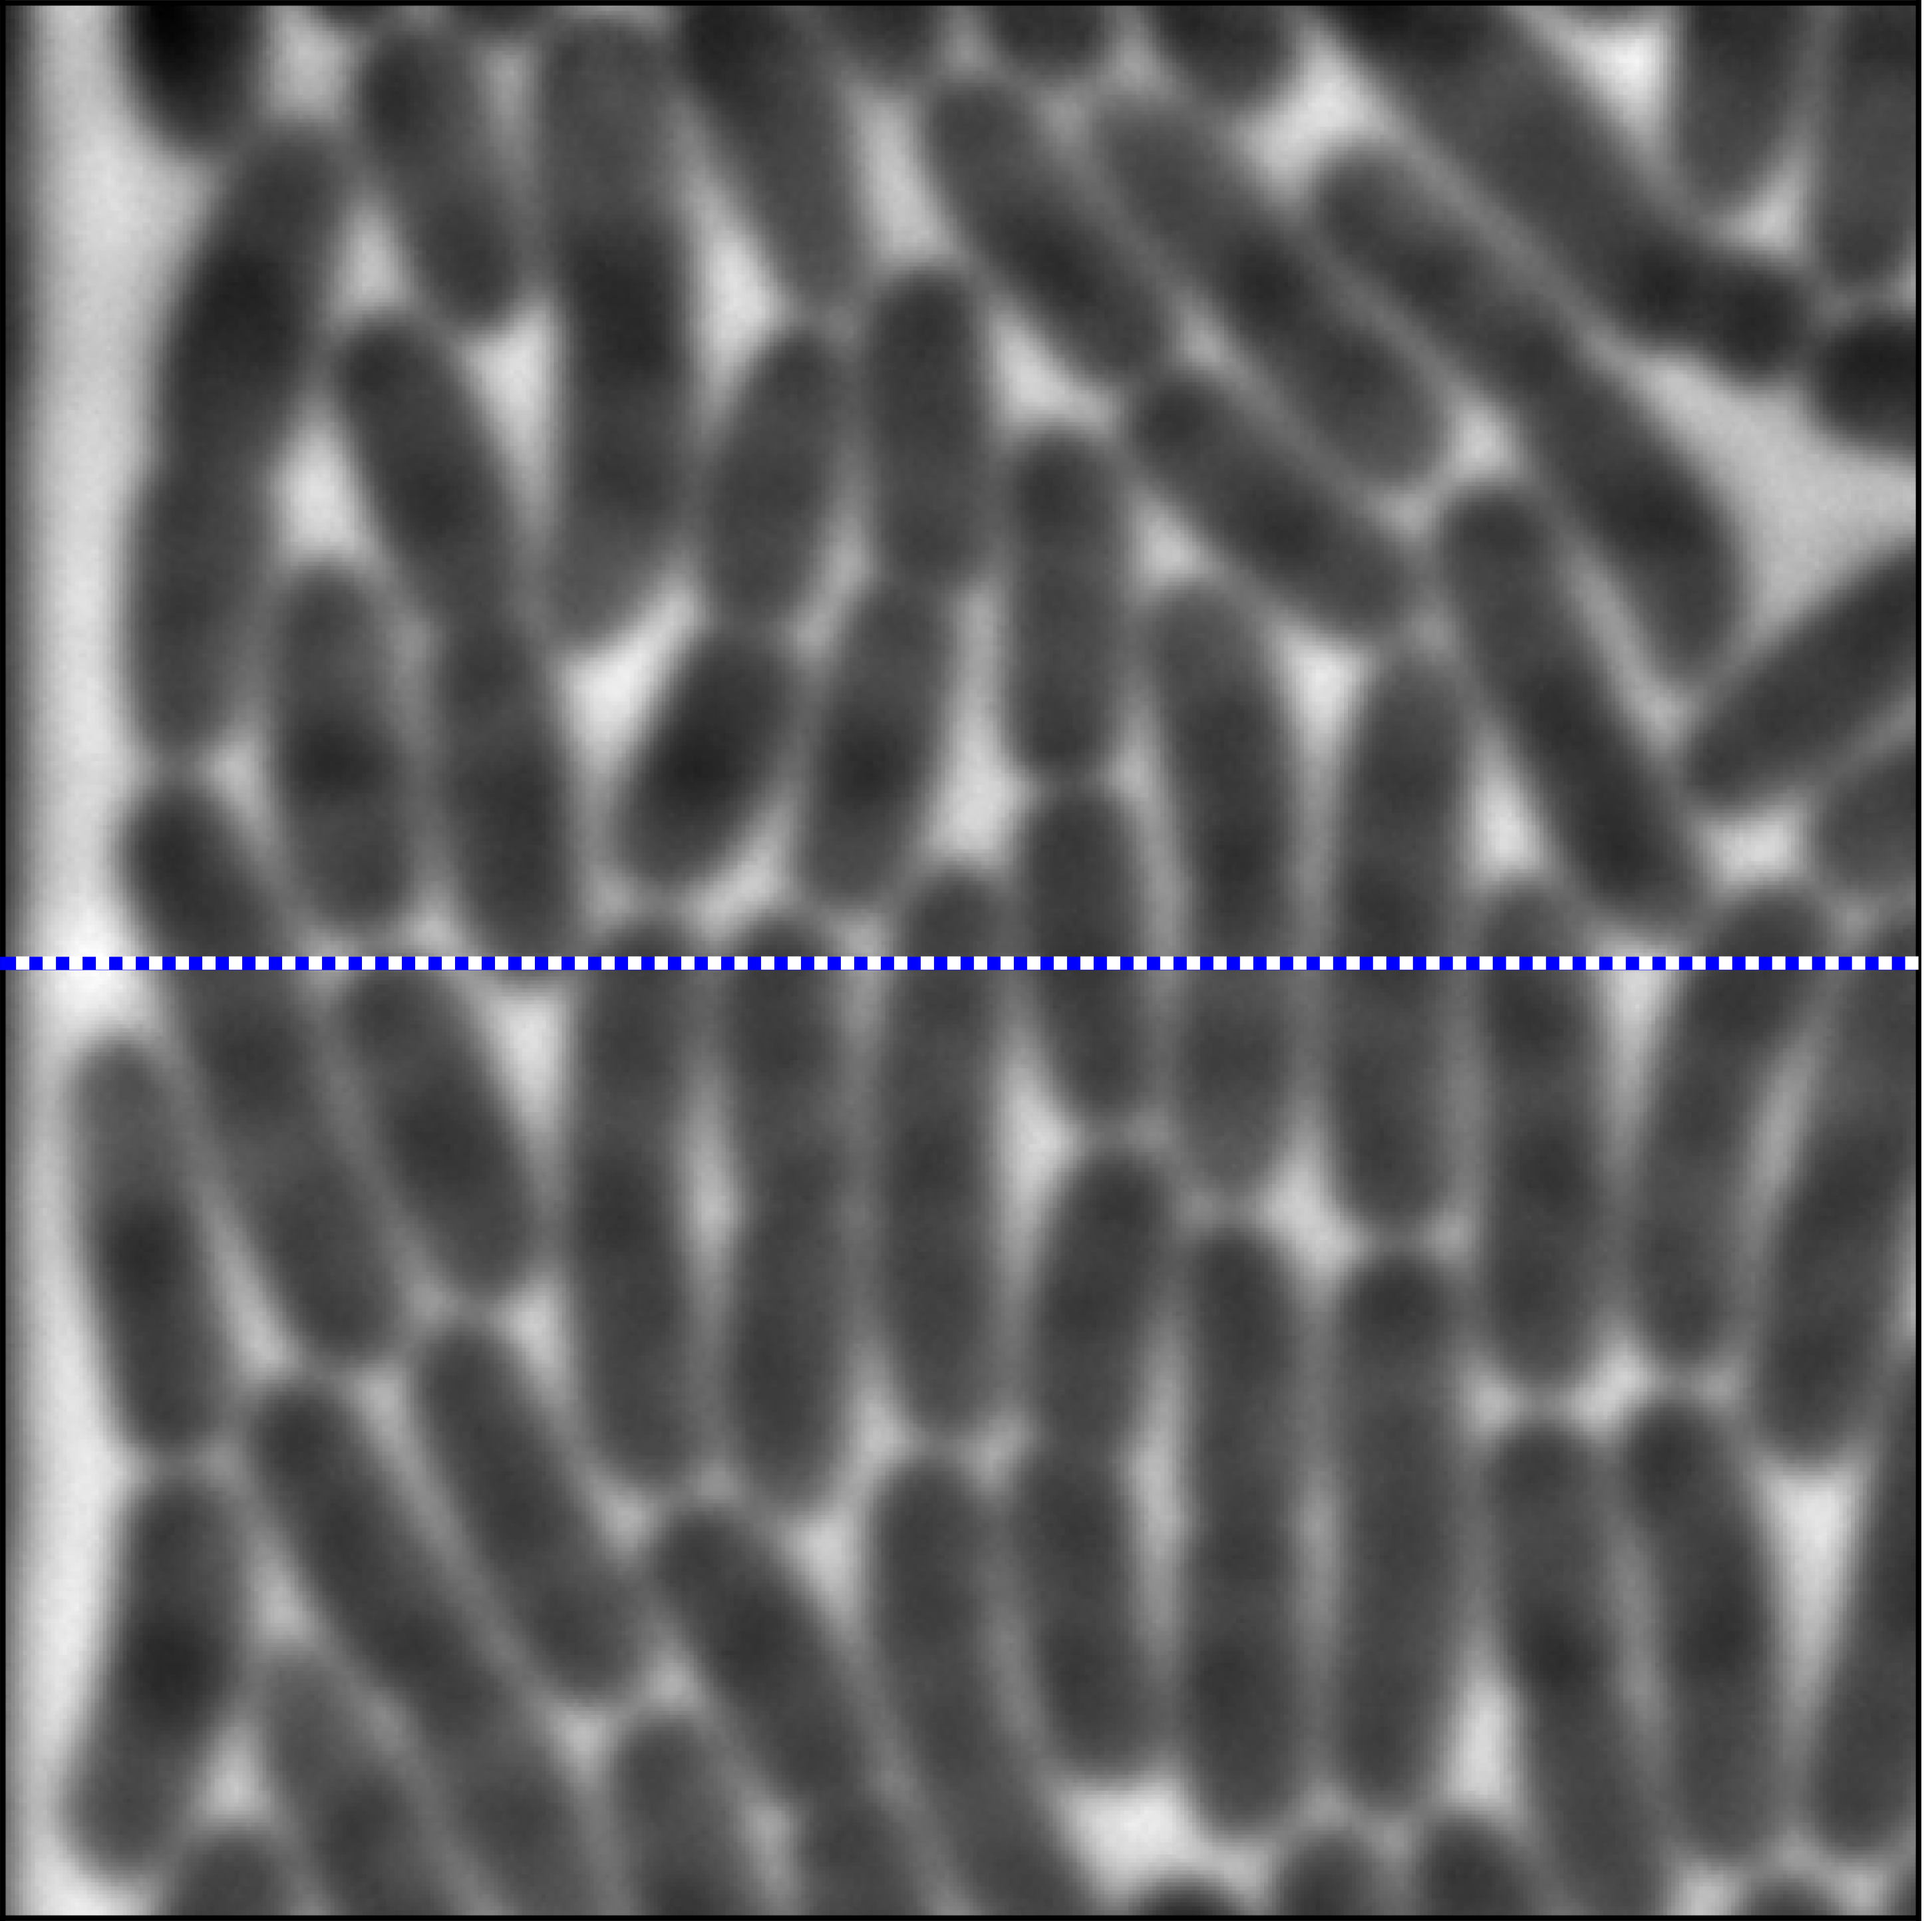
\includegraphics[width=2.5cm]{orimgmark.png}&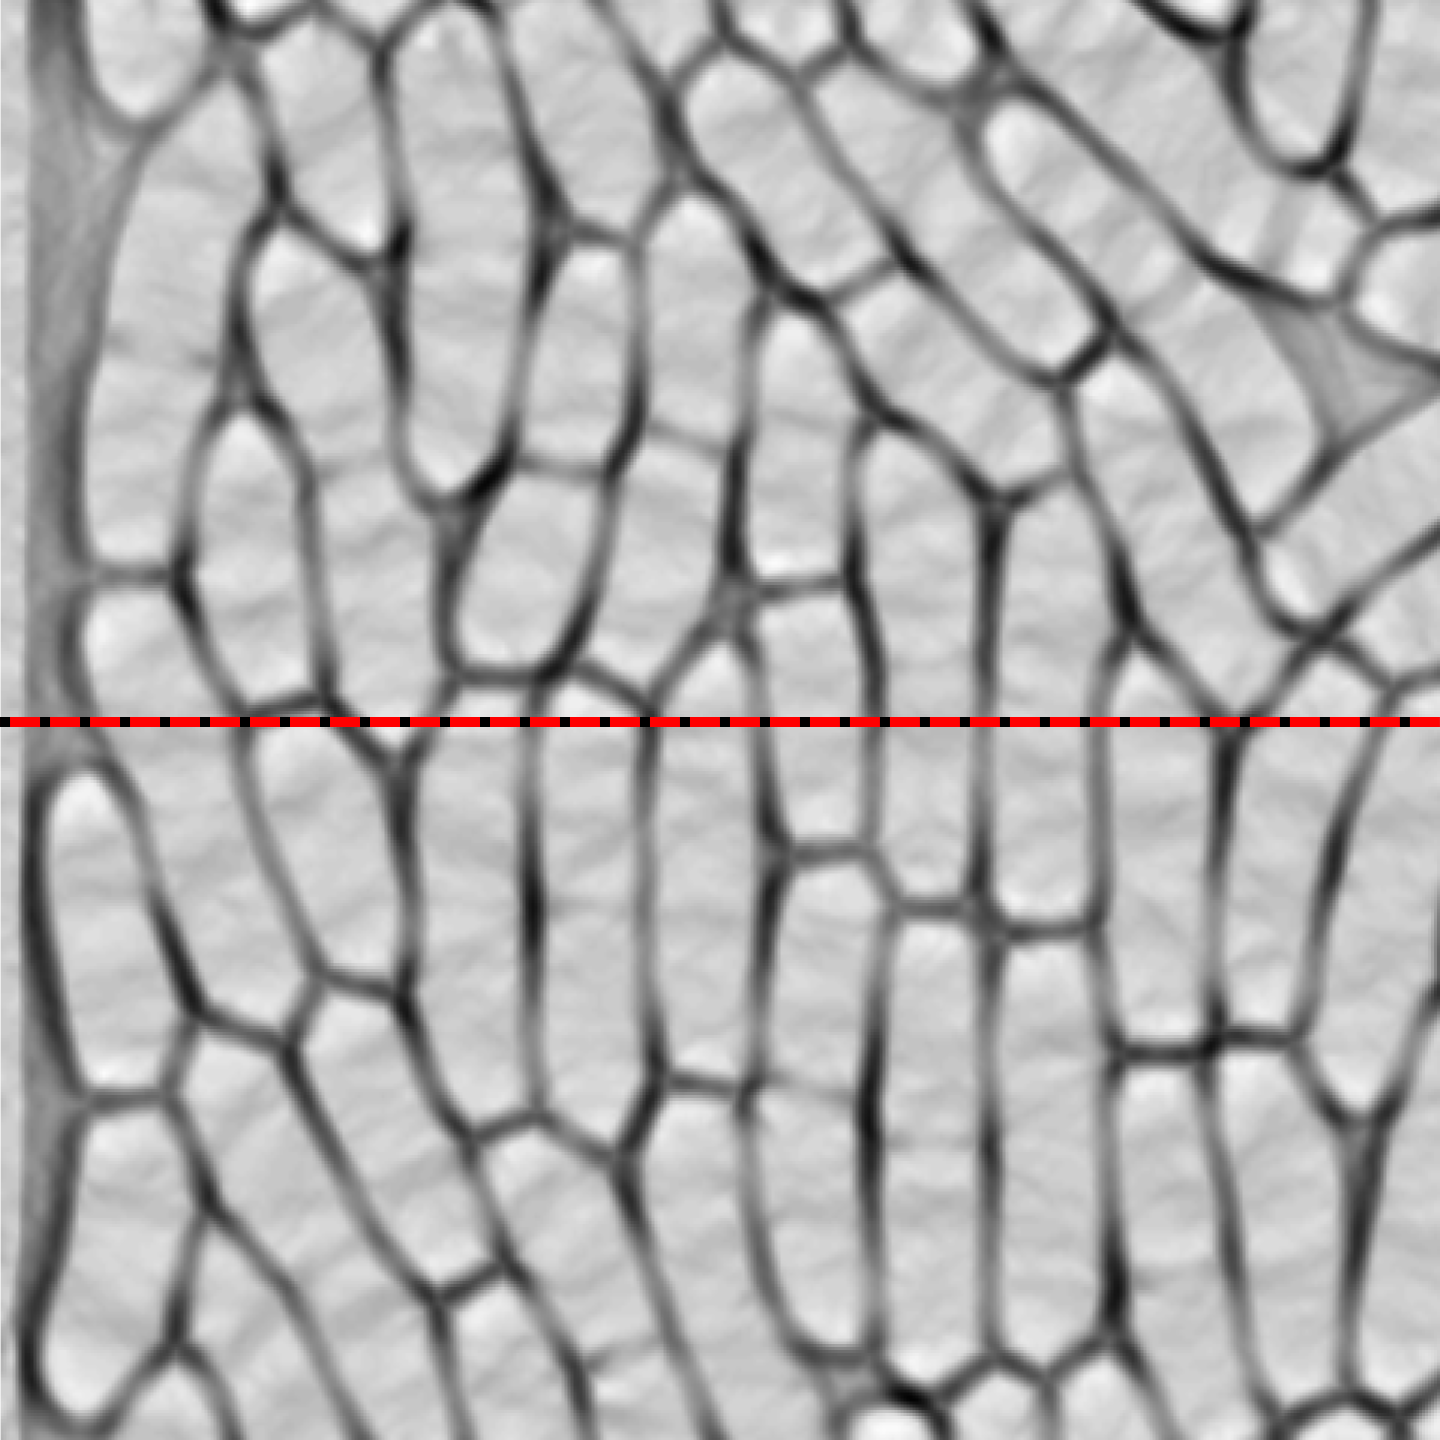
\includegraphics[width=2.5cm]{eigenmark.png}&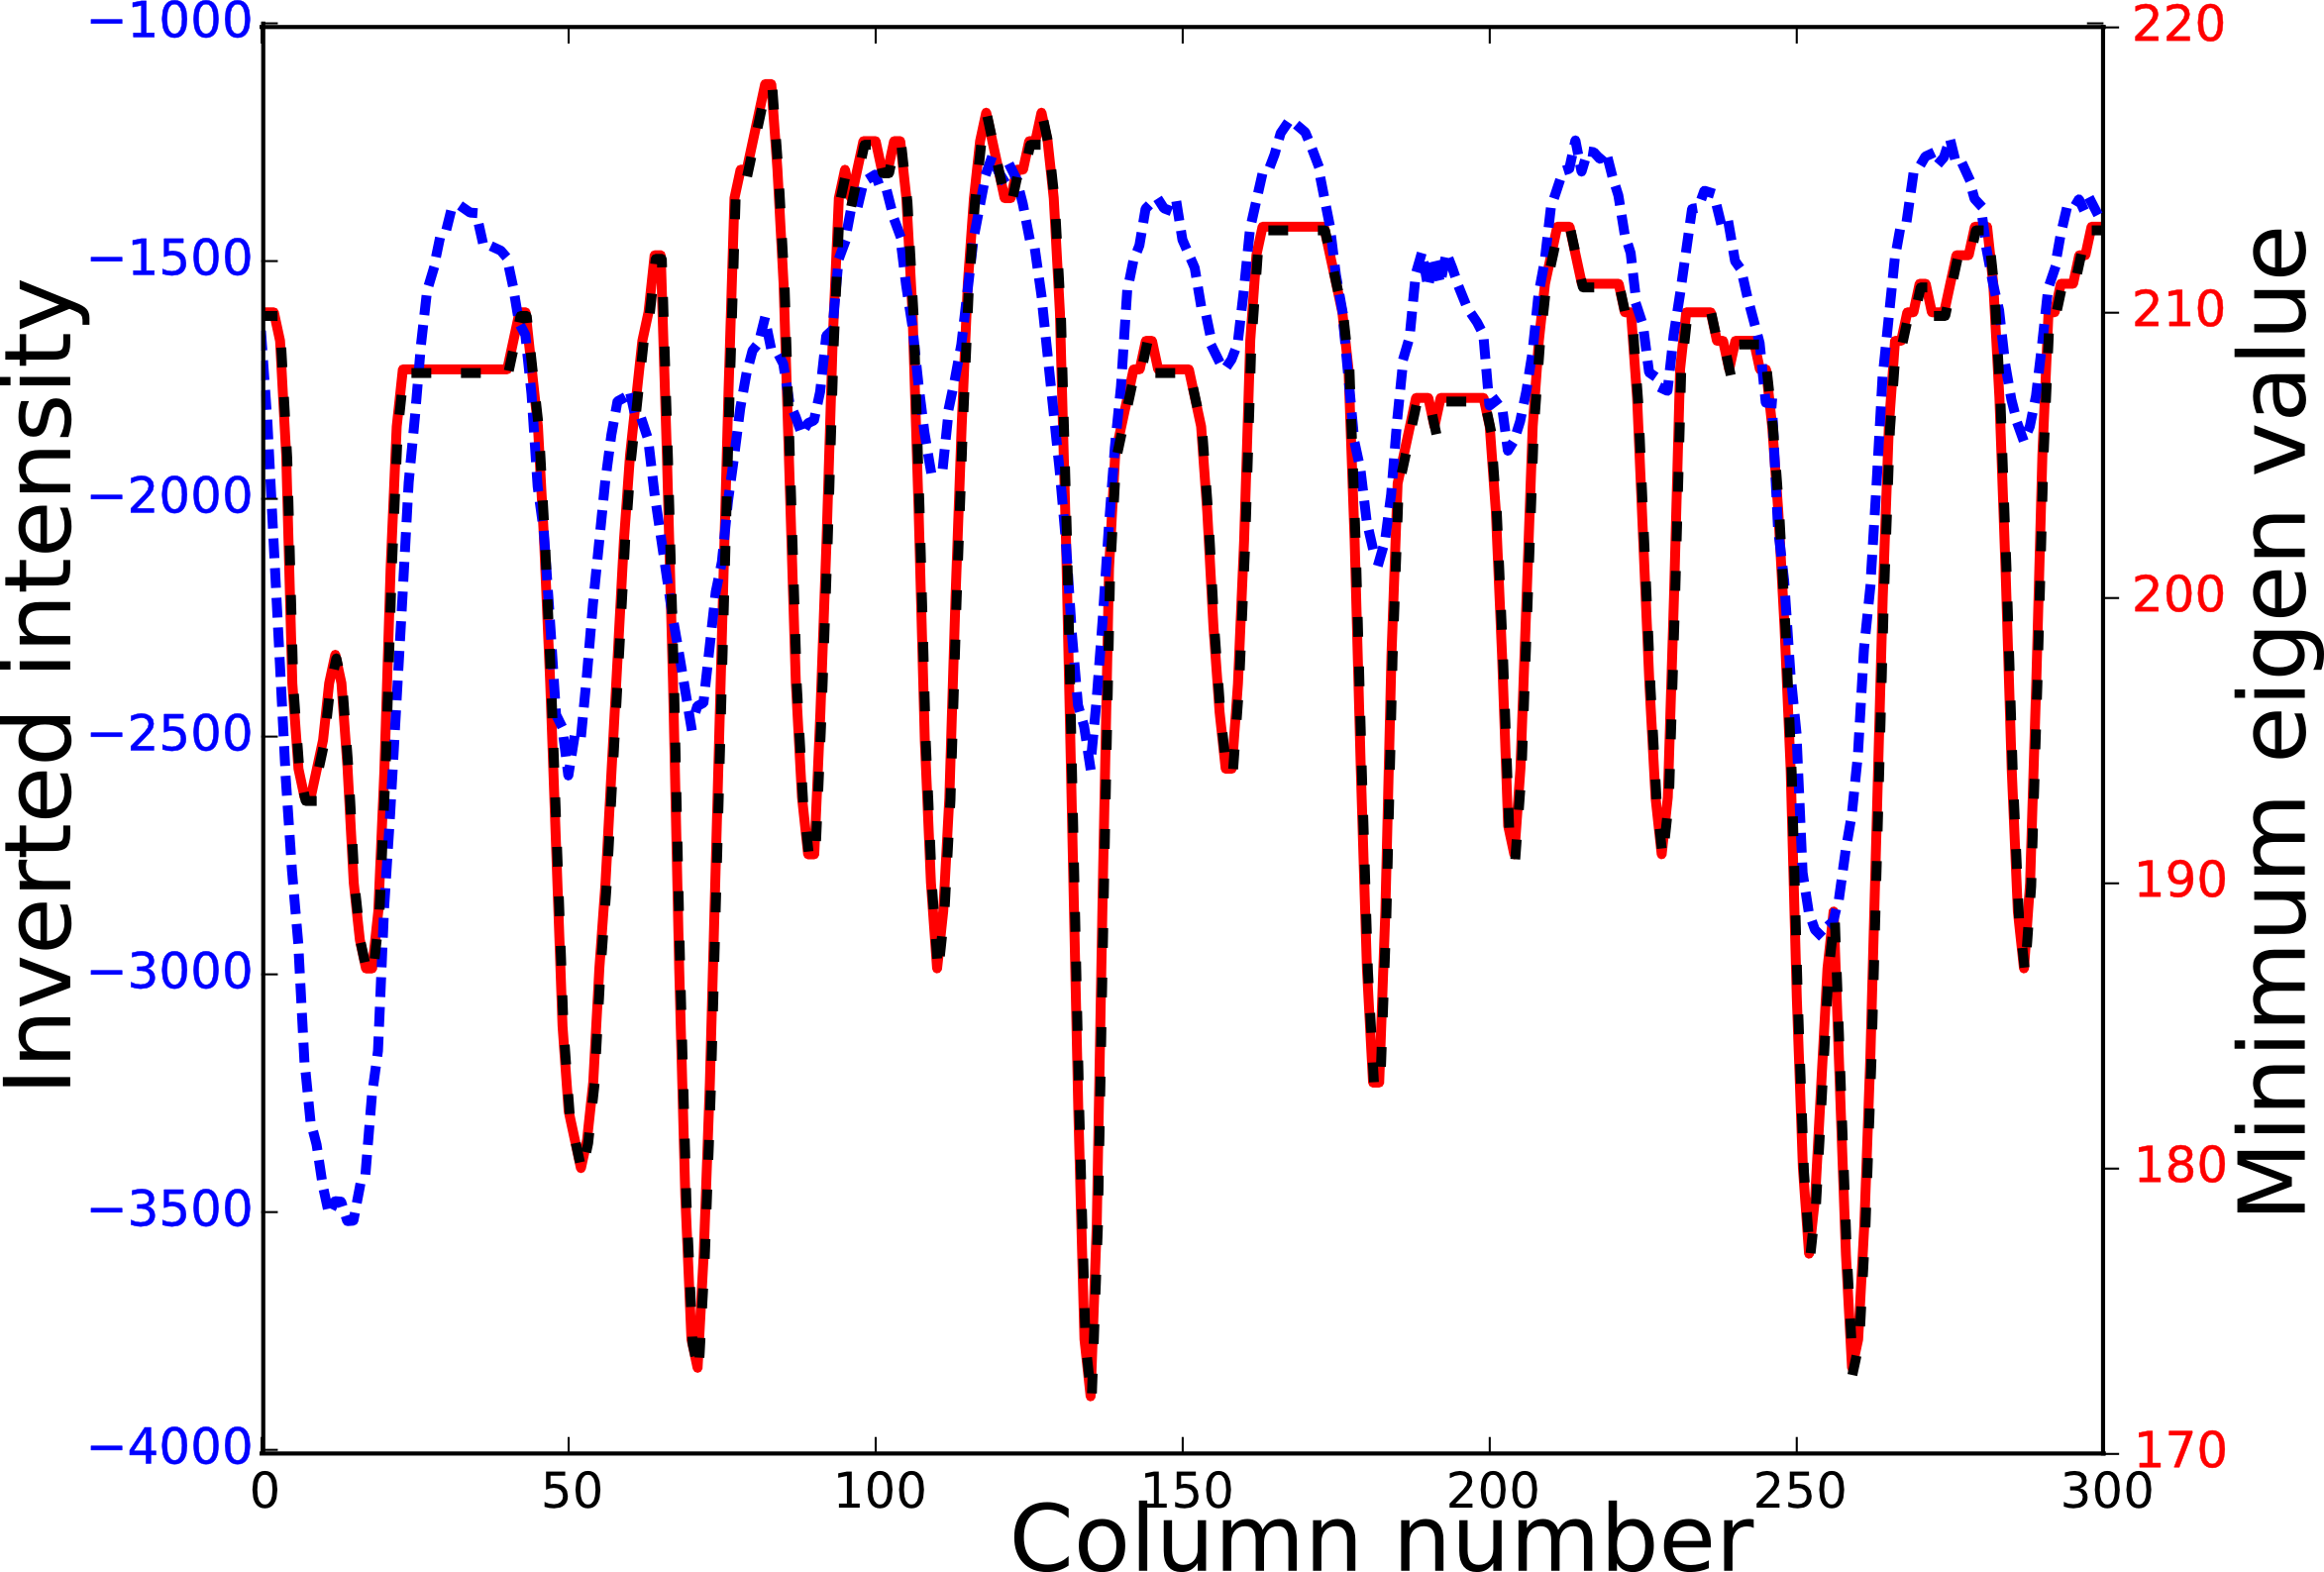
\includegraphics[width=2.5cm]{combineplots.png}
			\\
			a) & b) & c)
		\end{tabular}
		\caption{a) Original input image, b) curvature based contrast enhanced image and c) plot showing pixel values from the same row from a (red line), and b (blue line). Note that the plotted pixel values in c are inverted for display.}\label{fig:contrastenhance}
	\end{center}
\end{figure}


\subsection{Object Segmentation}
We used the presented curvature-based enhancement step to enhance the contrast in the images. Next, we segmented out the cells using a repeated thresholding approach. The contrast-enhanced image is an image with floating point values. In order to make the threshold computation easier, we normalized the image and quantized it to 256 intensity levels . A single threshold value was not sufficient to separate all individual cells, and watershed segmentation resulted in ambiguities in the positioning of the edges of the cells. We therefore used multiple thresholds and prior knowledge about the cell area and the cell shape, in the form of major and minor axes lengths,  to filter out the cells from background regions. 

For each threshold level, the image was labeled and each object fitted with an ellipse. The ellipse parameters are found using moments \cite{burgerprinciples2009} as follows. We create a matrix M
  
$M = \begin{bmatrix}
m_{02}&m_{11} \\
m_{11}&m_{20}
\end{bmatrix}$

\begin{equation}
\text{major axis} = 4 \times \sqrt{\frac{\lambda_1}{m_{00}}}
\end{equation}

\begin{equation}
\text{minor axis} = 4 \times \sqrt{\frac{\lambda_2}{m_{00}}}
\end{equation}

$\lambda_1$ and $\lambda_2$ are eigenvalues of moment matrix M,  $m_{pq}$ is the p, $q^{th}$ central moment in x and y axis respectively.  $m_{00}$ is $0^{th}$ central moment (area of the object). 

The ellipse parameters of individual objects were analyzed as follows; the objects were filtered based on the major and minor axis length to remove very large and very small regions. The major and minor axes lengths are given as parameter to the algorithm. For each object, a weight is calculated as follows and assigned to the object.

\begin{equation}
\textit{weight} = 0.5 \times \textit{residual area ratio} + 0.5 \times convexity 
\end{equation}

where the residual area ratio (RAR) is the ratio found as

\begin{equation}
\textit{RAR} = \frac{\textit{min(area, ellipse area) }}{\textit{max( area, ellipse area)}}  
\end{equation}

and convexity

\begin{equation}
\textit{convexity} = \frac{\textit{ area }}{\textit{area of convex hull of object}}  
\end{equation}

Ellipse area is found as

\begin{equation}
\textit{Ellipse area} = \frac{ \pi \times \textit{ major axis }\times \textit{minor axis}}{4}  
\end{equation}

From a computational point of view it is time-consuming to apply a threshold at all the 255 intensity levels and analyze the size and shape of every binary object present in the image. We have already seen that the cellular regions exhibit higher intensity values and edges between cells exhibit lower intensity values on the contrast-enhanced image. Thus we made the assumption that the histogram is bimodal, with the largest peak representing object and background pixels, while the smaller peak represents edges. We therefore started our repeated thresholding at the intensity value at the local minimum of the histogram (assuming this is well below the intensity of the cells), and set the ending threshold as the intensity at the largest peak. These values may change depending on the dataset, but proved robust on the four different datasets evaluated here.






\subsubsection{Subsubsection Heading Here}
Subsubsection text here.


% An example of a floating figure using the graphicx package.
% Note that \label must occur AFTER (or within) \caption.
% For figures, \caption should occur after the \includegraphics.
% Note that IEEEtran v1.7 and later has special internal code that
% is designed to preserve the operation of \label within \caption
% even when the captionsoff option is in effect. However, because
% of issues like this, it may be the safest practice to put all your
% \label just after \caption rather than within \caption{}.
%
% Reminder: the "draftcls" or "draftclsnofoot", not "draft", class
% option should be used if it is desired that the figures are to be
% displayed while in draft mode.
%
%\begin{figure}[!t]
%\centering
%\includegraphics[width=2.5in]{myfigure}
% where an .eps filename suffix will be assumed under latex, 
% and a .pdf suffix will be assumed for pdflatex; or what has been declared
% via \DeclareGraphicsExtensions.
%\caption{Simulation results for the network.}
%\label{fig_sim}
%\end{figure}

% Note that IEEE typically puts floats only at the top, even when this
% results in a large percentage of a column being occupied by floats.


% An example of a double column floating figure using two subfigures.
% (The subfig.sty package must be loaded for this to work.)
% The subfigure \label commands are set within each subfloat command,
% and the \label for the overall figure must come after \caption.
% \hfil is used as a separator to get equal spacing.
% Watch out that the combined width of all the subfigures on a 
% line do not exceed the text width or a line break will occur.
%
%\begin{figure*}[!t]
%\centering
%\subfloat[Case I]{\includegraphics[width=2.5in]{box}%
%\label{fig_first_case}}
%\hfil
%\subfloat[Case II]{\includegraphics[width=2.5in]{box}%
%\label{fig_second_case}}
%\caption{Simulation results for the network.}
%\label{fig_sim}
%\end{figure*}
%
% Note that often IEEE papers with subfigures do not employ subfigure
% captions (using the optional argument to \subfloat[]), but instead will
% reference/describe all of them (a), (b), etc., within the main caption.
% Be aware that for subfig.sty to generate the (a), (b), etc., subfigure
% labels, the optional argument to \subfloat must be present. If a
% subcaption is not desired, just leave its contents blank,
% e.g., \subfloat[].


% An example of a floating table. Note that, for IEEE style tables, the
% \caption command should come BEFORE the table and, given that table
% captions serve much like titles, are usually capitalized except for words
% such as a, an, and, as, at, but, by, for, in, nor, of, on, or, the, to
% and up, which are usually not capitalized unless they are the first or
% last word of the caption. Table text will default to \footnotesize as
% IEEE normally uses this smaller font for tables.
% The \label must come after \caption as always.
%
%\begin{table}[!t]
%% increase table row spacing, adjust to taste
%\renewcommand{\arraystretch}{1.3}
% if using array.sty, it might be a good idea to tweak the value of
% \extrarowheight as needed to properly center the text within the cells
%\caption{An Example of a Table}
%\label{table_example}
%\centering
%% Some packages, such as MDW tools, offer better commands for making tables
%% than the plain LaTeX2e tabular which is used here.
%\begin{tabular}{|c||c|}
%\hline
%One & Two\\
%\hline
%Three & Four\\
%\hline
%\end{tabular}
%\end{table}


% Note that the IEEE does not put floats in the very first column
% - or typically anywhere on the first page for that matter. Also,
% in-text middle ("here") positioning is typically not used, but it
% is allowed and encouraged for Computer Society conferences (but
% not Computer Society journals). Most IEEE journals/conferences use
% top floats exclusively. 
% Note that, LaTeX2e, unlike IEEE journals/conferences, places
% footnotes above bottom floats. This can be corrected via the
% \fnbelowfloat command of the stfloats package.




\section{Conclusion}
The conclusion goes here.





% if have a single appendix:
%\appendix[Proof of the Zonklar Equations]
% or
%\appendix  % for no appendix heading
% do not use \section anymore after \appendix, only \section*
% is possibly needed

% use appendices with more than one appendix
% then use \section to start each appendix
% you must declare a \section before using any
% \subsection or using \label (\appendices by itself
% starts a section numbered zero.)
%


\appendices
\section{Proof of the First Zonklar Equation}
Appendix one text goes here.

% you can choose not to have a title for an appendix
% if you want by leaving the argument blank
\section{}
Appendix two text goes here.


% use section* for acknowledgment
\section*{Acknowledgment}


The authors would like to thank...


% Can use something like this to put references on a page
% by themselves when using endfloat and the captionsoff option.
\ifCLASSOPTIONcaptionsoff
  \newpage
\fi



% trigger a \newpage just before the given reference
% number - used to balance the columns on the last page
% adjust value as needed - may need to be readjusted if
% the document is modified later
%\IEEEtriggeratref{8}
% The "triggered" command can be changed if desired:
%\IEEEtriggercmd{\enlargethispage{-5in}}

% references section

% can use a bibliography generated by BibTeX as a .bbl file
% BibTeX documentation can be easily obtained at:
% http://www.ctan.org/tex-archive/biblio/bibtex/contrib/doc/
% The IEEEtran BibTeX style support page is at:
% http://www.michaelshell.org/tex/ieeetran/bibtex/
\bibliographystyle{IEEEtran}
\bibliography{sample}

\end{document}


